\documentclass[11pt]{article}

\usepackage[margin=1in]{geometry}
\usepackage{amsmath, amssymb, amsthm}
\usepackage{algorithm}
\usepackage{algpseudocode}
\usepackage{hyperref}
\usepackage{enumitem}
\usepackage{booktabs}
\usepackage{tikz}
\usetikzlibrary{arrows.meta,positioning}

\title{Notes on the Artificial Neuron}
\author{}
\date{}

\begin{document}
\maketitle

\section{Motivation}

The function-approximation notes ended with linear methods,
$\hat v(s\mid\mathbf{w}) = \mathbf{w}\cdot\phi(s)^{\top}$, where all of the
nonlinearity had to be hand-engineered into the fixed feature map $\phi$
(polynomial terms, Fourier terms, tiles). A \textbf{neural network}
instead \emph{learns} that nonlinearity jointly with the weights, and its
elementary building block is the \textbf{artificial neuron}: a single
unit that takes a weighted sum of its inputs, adds a bias, and passes the
result through a fixed nonlinear \textbf{activation function}. Stacking
many such neurons in layers is what turns a linear-in-features model into
a general nonlinear function approximator $\hat v(s;\theta)$ or
$\hat q(s,a;\theta)$ — this section builds the single-unit model; later
sections stack it into a network.

\section{The model}

Given an input vector $x = (x_1, \dots, x_n) \in \mathbb{R}^n$, a weight
vector $w = (w_1, \dots, w_n) \in \mathbb{R}^n$, and a scalar bias $b$, the
neuron first computes a weighted sum called the \textbf{net input} (or
\textbf{pre-activation}):

\[
    z = w \cdot x + b = \sum_{i=1}^{n} w_i x_i + b = w^{\top} x + b,
\]

and then applies an \textbf{activation function} $g: \mathbb{R} \to
\mathbb{R}$ to produce the neuron's output (\textbf{activation}):

\[
    a = g(z) = g\big(w^{\top}x + b\big).
\]

The bias $b$ is often folded into $w$ by appending a constant input
$x_0 = 1$ with weight $w_0 = b$, giving the compact form
$z = w^{\top}x$ with $x = (1, x_1, \dots, x_n)$ and $w = (b, w_1, \dots,
w_n)$ — the same trick used to fold an intercept into a linear-regression
design matrix.

\begin{center}
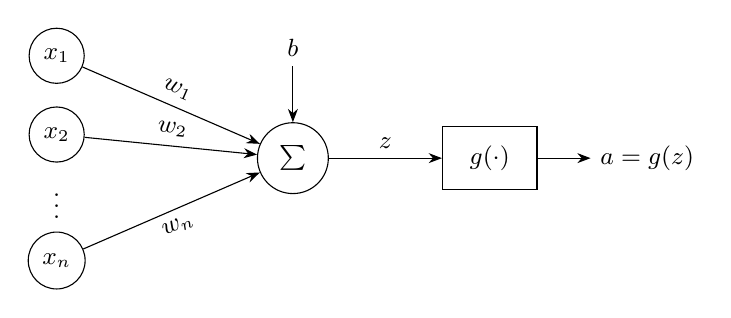
\begin{tikzpicture}[
    every node/.style={font=\small},
    input/.style={circle, draw, minimum size=0.7cm},
    sum/.style={circle, draw, minimum size=0.9cm},
    >=Stealth
]
    \node[input] (x1) at (0,1.5) {$x_1$};
    \node[input] (x2) at (0,0.5) {$x_2$};
    \node at (0,-0.3) {$\vdots$};
    \node[input] (xn) at (0,-1.1) {$x_n$};
    \node[sum] (z) at (3,0.2) {$\sum$};
    \node (b) at (3,1.6) {$b$};
    \node[draw, minimum width=1.2cm, minimum height=0.8cm] (g) at (5.5,0.2) {$g(\cdot)$};
    \node (out) at (7.5,0.2) {$a = g(z)$};

    \draw[->] (x1) -- node[above,sloped]{$w_1$} (z);
    \draw[->] (x2) -- node[above,sloped]{$w_2$} (z);
    \draw[->] (xn) -- node[below,sloped]{$w_n$} (z);
    \draw[->] (b) -- (z);
    \draw[->] (z) -- node[above]{$z$} (g);
    \draw[->] (g) -- (out);
\end{tikzpicture}
\end{center}

\section{Activation functions}

The choice of $g$ determines what the neuron can express and how it
behaves under gradient-based learning.

\begin{center}
\begin{tabular}{@{}p{2.6cm}p{5.0cm}p{5.6cm}@{}}
\toprule
Name & $g(z)$ & Notes \\
\midrule
Linear (identity) & $g(z) = z$ & $a$ is just $w^{\top}x+b$; a single such
neuron \emph{is} linear regression, and is exactly the linear function
approximator $\hat v = \mathbf{w}\cdot\phi(s)^\top$ from the previous
notes. \\
Step (Heaviside) & $g(z) = \begin{cases} 1 & z \geq 0 \\ 0 & z < 0
\end{cases}$ & The original McCulloch--Pitts / perceptron
nonlinearity; not differentiable, so unusable with gradient descent. \\
Sigmoid (logistic) & $g(z) = \dfrac{1}{1+e^{-z}}$ & Squashes to $(0,1)$;
$g'(z) = g(z)\big(1-g(z)\big)$. A single sigmoid neuron is exactly logistic
regression. \\
Tanh & $g(z) = \tanh(z) = \dfrac{e^{z}-e^{-z}}{e^{z}+e^{-z}}$ & Squashes to
$(-1,1)$, zero-centered (often trains better than sigmoid);
$g'(z) = 1 - \tanh^2(z)$. \\
ReLU & $g(z) = \max(0, z)$ & $g'(z) = \mathbb{1}[z>0]$ (subgradient $0$ at
$z=0$); avoids the vanishing-gradient problem of sigmoid/tanh for large
$|z|$ and is the default in most modern hidden layers. \\
\bottomrule
\end{tabular}
\end{center}

\section{A single neuron as a function approximator}

With $g$ the identity, the neuron reduces exactly to the linear
approximator of the previous notes, $\hat v(s\mid w) = w^{\top}\phi(s)$.
With $g$ a sigmoid, the same unit becomes logistic regression — a natural
model when the target is a probability (e.g.\ estimating a policy's
probability of taking an action, $\pi(a\mid s) \approx g(w^\top\phi(s,a))$)
rather than a real-valued prediction. In both cases the neuron is a linear
model in disguise: all of its representational power still comes from the
fixed feature map $\phi$ feeding it, exactly as in Section~4 of the
function-approximation notes. Nonlinear representational power only
appears once neurons are \emph{composed} — the output of one layer of
neurons feeding as $x$ into another layer — which is what turns fixed
features $\phi(s)$ into features the network learns for itself.

\section{Learning: gradient descent on a single neuron}

Treat $(w, b)$ as the parameter vector $\theta$ and reuse the SGD
machinery from the function-approximation notes: given a target $U_t$ for
the neuron's output at input $x_t$, and squared-error loss
$L = \frac{1}{2}\big[U_t - a_t\big]^2$ with $a_t = g(z_t)$,
$z_t = w^\top x_t + b$, the chain rule gives

\[
    \frac{\partial L}{\partial w_i} = -\big[U_t - a_t\big]\, g'(z_t)\, x_{t,i},
    \qquad
    \frac{\partial L}{\partial b} = -\big[U_t - a_t\big]\, g'(z_t),
\]

so the SGD update is

\[
    w_i \leftarrow w_i + \alpha \big[U_t - a_t\big]\, g'(z_t)\, x_{t,i}, \qquad
    b \leftarrow b + \alpha \big[U_t - a_t\big]\, g'(z_t).
\]

This is precisely the general update
$\mathbf{w} \leftarrow \mathbf{w} + \alpha[U_t - \hat v(S_t\mid\mathbf{w})]
\nabla \hat v(S_t\mid\mathbf{w})$ from the function-approximation notes,
specialized to $\hat v(s\mid w) = g(w^\top\phi(s))$, so
$\nabla \hat v = g'(z)\,\phi(s)$. For the linear activation ($g(z)=z$,
$g'(z)=1$) this collapses back to the plain linear-approximator update;
the extra factor $g'(z_t)$ is the only change a nonlinear activation
introduces at a single neuron, and it is exactly the local term that the
backpropagation algorithm chains together across layers once neurons are
stacked into a network.

\begin{algorithm}[h]
\caption{SGD training of a single neuron}
\begin{algorithmic}[1]
\State Initialize $w, b$ (e.g.\ small random values); fix $\alpha$ and activation $g$
\For{each sample $(x_t, U_t)$}
    \State $z_t \leftarrow w^\top x_t + b$
    \State $a_t \leftarrow g(z_t)$
    \State $\delta_t \leftarrow U_t - a_t$
    \State $w \leftarrow w + \alpha\, \delta_t\, g'(z_t)\, x_t$
    \State $b \leftarrow b + \alpha\, \delta_t\, g'(z_t)$
\EndFor
\end{algorithmic}
\end{algorithm}

\section{From one neuron to a network}

A single neuron, whatever $g$ is chosen, can only separate its input space
along one hyperplane $w^\top x + b = 0$ (linearly, for the step/sigmoid
case) — it cannot represent, e.g., XOR. Feeding the outputs of a layer of
$m$ neurons as the input vector to a next layer of neurons is what allows
the composition of many such hyperplane-based decisions to approximate
arbitrary nonlinear functions (a \textbf{multi-layer perceptron}), with
$v_\pi$ or $q_\pi$ played by the whole network rather than a single unit,
and $\theta$ now denoting every layer's weights and biases together — the
setting used later for approximators such as DQN.

\section{Reference}

Sutton, R.\ S., \& Barto, A.\ G.\ \emph{Reinforcement Learning: An
Introduction}, 2nd ed., Section~9.7 (Nonlinear Function Approximation:
Artificial Neural Networks). Goodfellow, I., Bengio, Y., \& Courville, A.\
\emph{Deep Learning}, Ch.~6 (Deep Feedforward Networks), for the neuron
model and activation functions in more depth.

\end{document}
